\documentclass{article}
\usepackage[utf8]{inputenc}
\usepackage{graphicx}
\newcommand\tab[1][1cm]{\hspace*{#1}}

\title{TI}
\author{Sebastian Benkel}
\date{January 2017}

\begin{document}

1. Welche zwei Hauptaufgaben hat ein Betriebssystem?
\\
\\
Abstraktion von Ger\"ateeigenschaften(Alle Drucker lassen sich gleich verwenden, Standartinterfaces, etc.)

Unterst\"utzung des Mehrbenutzerbetriebs(Betriebsmittelverwaltung, Zuteilungsstrategien, etc)
\\
\\
2. Was ist ein Prozess?
\\
\\
Ein Programm in ausf\"uhrung(Kontrollfaden)
\\
\\
3. Wie ist ein Unix-Dateisystem strukturiert? Wie können Dateien darin (eindeutig) aufgefunden werden?
\\
\\
Es besteht aus Langlebigen Datenobjekten, die \"uber ihren eindeutigen Namen(Vollständige Dateinamen sind Pfadnamen vom Wurzelverzeichnis abwärts)(mehrere solcher Namen pro Datei m\"oglich) identifiziert werden k\"onnen. Die Struktur ist hierarchisch und Baumartig, l\"asst aber mehr als einen Pfad zur Datei zu.
\\
\\
4. Was ist ein symbolic link?
\\
\\
Ein Symbolic Link ist ein Pfadverweis auf eine Datei oder einen Ordner. Wird die Datei entfernt zeigt der Link an eine nicht existente Adresse.
\\      
\\
5. Ist das Unix-Dateisystem wirklich ein Baum? Begründung.
\\
\\
Nein, in einem Baum kann es keine zwei Wege auf die selbe Stelle geben. Im Unix-Dateisystem geht dies f\"ur Dateien(Hard Links)(Nicht f\"ur Ordner um Rekursion zu verhindern).
\\
\\
6. Welche Zugriffsrechte kann man auf eine Unix-Datei haben? Welche Dateiattribute steuern
dies, und wie?
\\
\\
Es gibt Read(lesen des Dateiinhalts. einsicht bei Ordnern), Write(ver\"andern des Dateiinhalts, Eintr\"age \"andern bei Ordnern), und Execute(ausf\"uhren der Datei als Programm, Zugriff auf Inhalt bei Ordnern) Rechte. diese werden in den Atributen der Datei vermerkt(f\"ur besitzer, Gruppe und Welt). \"Anderbar mit chmod
\\
\\
7. Welche Vorteile bietet es, auf Geräte in Unix wie auf Dateien zuzugreifen? Was versteht
man unter Ein-/Ausgabeumlenkung?
\\
\\
Textausgaben werden standartm\'a\ss ig in eine \"{}Standart-Ausgabedatei\"{} (das aktive Terminal(''stdout'')) geschrieben. diese kann durch andere Dateien ersetzt werden, so das Textausgabe direkt in Dateien umgelenkt werden k\"onnen.($>,>>.|$).
Dateiinhalt kann so an funktionen(sort, etc) \"ubergeben werden.
\\
\\
8. Welche Aufgabe hat ein Kommando-Interpreter (z.B. in Unix der Shell)?
\\
\\
Befehle entgegen zunehmen und umzusetzen, Prozesse abzubrechen, neue Prozesse aufzusetzen, generell Usereingaben umzusetzen.
\\
\\
9. Was machst Du, wenn Dir die genaue Semantik eines Unix-Kommandos entfallen ist?
\\
\\
\$ man Komandoname liefert die manpage
\\
\\
10. bla sei ein ausführbares Programm. Was ist der Unterschied zwischen dem Aufruf bla und
dem Aufruf bla \& in der Shell? Welche Auswirkungen hat dies, wenn bla von Standard
Input liest bzw. auf Standard Output schreibt? Gegeben sei der in Abbildung 1 dargestellte
Prozessbaum. Wie ändert er sich nach Eingeben der folgenden Kommandofolge im Shell?
init
bash
Abbildung 1: Prozessbaum
sleep 1000 \&
emacs \&
bash
date

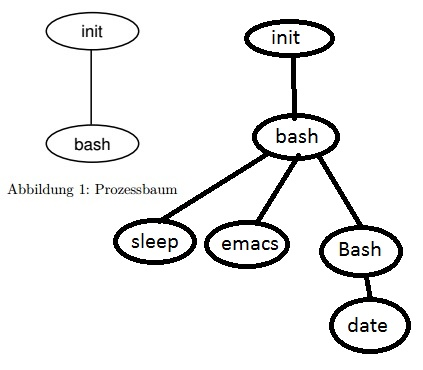
\includegraphics{Ti1.jpeg}
\\
\\
Der Aufruf bla \"ubergibt die Kontrolle der Komandozeile an den gestarteten Prozess, so das eingegebene Befehle nicht mehr ber\"ucksichtigt werden(bis auf Signale wie ctl-...). Der Aufruf bla /& startet bla als Hintergrundprozess und die Kontrolle der Komandozeile wird nicht abgegeben. Eingaben werden weiter angenommen. Textausgaben von bla werden im Terminal ausgegeben(sehr un\"ubersichtlich). 
\\
\\
11. Nenne drei Beispiele für Informationen, die der Betriebssystemkern über einen Prozess
wissen muss.
\\
\\
Vaterprozess(PPID), Jobnummer(PID), Besitzer(UID),
\\
\\
12. Was ist eine Pipe?
\\
\\
Eine Pipe ist ein Buffer der die Ausgabe eines Prozesses mit der Eingabe eines Anderen Prozesses verbindet(stdin, stdout).
\\
\\
13. Wie macht man ein soeben editiertes Shell-File ausführbar?
\\
\\
chmod 1/chmod3/chmod5,chmod7...
\\
\\
14. In welche Bereiche (Segmente) ist der (virtuelle) Adressraum eines Programms in Ausführung in Unix unterteilt, und welche Eigenschaften kennzeichnen sie?
\\
\\
Text - hier liegt der code des Programms, sollte read-only sein.

Daten - hier liegen die (in Java, C++ durch  new) globalen vriablen des Programms, kann dynamisch erweitert werden(read + write)

Stack - hier wird der Status bei Prozeduraufrauf gerettet, die Parameter der Prozedur sowie Lokale Variablen der Prozedur (wächst/schrumpft dynamisch nach Bedarf) Es gibt einen Stackpointer um das Oberste Element anzuzeigen.(read + write)

Sie sind auf virtuelle Adressen abgebildet, d.h. werden im Arbeitsspeicher darauf gemapt.


Ungenutze Adressen - Hier liegt nichts, und es kann auch nicht zugrgriffen werden.
\\
\\
15. Wozu wird der Stack verwendet?
\\
\\
 hier liegt der Status(die Parameter der Prozedur sowie Lokale Variablen der Prozedur(wächst/schrumpft dynamisch nach Bedarf)). Es gibt einen Stackpointer um das Oberste Element anzuzeigen.
\\
\\
16. Welchem Zweck dienen Bibliotheken (Libraries)?
\\
\\
Libraries sind fertige Programmteile die einfach in ein Programm eingebettet werden um von ihnen genutzt zu werden(weniger schreibarbeit).
\\
\\
17. Welche Aufgabe erfüllt ein Linker?
\\
\\
Ein Linker erzeugt aus zusammengeh\"orenden .o Dateien eine Executable(Programm), mit gemeinsamem Adressraum und relativen call-adressen(call main() $\rightarrow$ call -116).
\\
\\
18. Wozu wird beim Assemblieren eine Symboltabelle angelegt?
\\
\\
Die Symboltabelle organisiert die Nutzung gemeinsamer Funktionen und Variablen. Wenn sie fertig gef\"ullt ist, beinhaltet sie einen Eintrag für jedes „sichtbare“ Symbol, bestehend aus:

\tab • Name des Symbols durch Verweis auf Startbyte in Stringtabelle

\tab • Typ (+Adresse)

Genutzt wird sie dann um Funktions- und Variablenaufrufe im Code durch relative Aufrufe zu ersetzen. Variablen werden an Adresse im Datensegment verlinkt. Um \"Uberladung bei Funktionen zu erm\"oglichen nutzt sie Namemangling(Parameterangaben am Namensende). Die eigentlichen Methodennamen liegen auf der Stringtabelle.  Wenn Das Programm fertig \"ubersetzt ist, kann die Symboltabelle, Stringtabelle und die Text/Data Relocation Tabelle gel\"oscht werden.
\\
\\
19. Welchen Vorteil hat es, Bibliotheken mit Position Independent Code zu versehen?
\\
\\
Der Code kann ausgef\"uhrt werden, auch wenn er nicht in der Originalzeile liegt. Library files werden von vielen Klassen parallel eingebunden und m\"ussen so nicht in jedem Programm in der selben zeile liegen.
\\
\\
20. Durch welche „Qualitätsmerkmale“ sollten Betriebssysteme gekennzeichnet sein? Nenne
Beispiele für konkurrierende Anforderungen.
\\
\\
Zuverlässigkeit:

\tab • Korrektheit - Verfügbarkeit

\tab • Sicherheit - Fehlertoleranz

\tab • Verfügbarkeit

\tab • Fehlertoleranz

\tab • Robustheit

Benutzerfreundlichkeit:

\tab • Verständlichkeit

\tab • Angemessenheit - Verständlichkeit

\tab • Vernünftiges Fehlerverhalten

Wartbarkeit und Flexibilität:

\tab • Testbarkeit

\tab • Erweiterbarkeit

\tab • Adaptierbarkeit

\tab • Portabilität

Leistungsfähigkeit:

\tab • Effektivität

\tab • Effizienz

Kosten - gegen alles
\\
\\
21. Worin unterscheidet sich der Kernel-Mode vom User-Mode (in Unix)? Warum wird diese
Unterscheidung getroffen?
\\
\\
Der Kermelmode hat seinen eigenen Adressraum(Text, Daten, Stack) den nur er betreten darf.

Eigenen Betriebssystem-Code den nur er ausf\"uhren darf. Dieser beinhaltet erweiterte funktionalit\"aten, eigene Maschineninstruktionen, er kann interupts unterdr\"ucken/aufschieben.

\\
\\
22. Was passiert in etwa bei einem Systemaufruf? (Reihenfolge der Arbeitsschritte.)
\\
\\
Das programm das den CPU benutzt wird pausiert und sein Zustand (User-Stack-Pointer (usp) auf den Kernel-Stack,
Register auf den Kernel-Stack (⇒ Kontext retten)) gerettet. Ggf. werden beim Interrupthandler interrupts Ausmaskiert(unterdr\"uckt), dann wird der Systemaufruf im Kernelmode abgearbeitet, es erfolgt ggf. Prozessumschaltung & Signalauslieferung, der Kernel-Stack wird aufgeräumt, es geht zur\"uck in den User-Mode, der User-Stack wird aufgeräumt und es geht zurück ins Anwendungsprogramm.
\\
\\
23. Was ist ein Interrupt? Nenne Beispiele für mögliche Interrupt-Quellen. Warum werden sie
unterschiedlich priorisiert? Wie wird ein Interrupt in etwa behandelt?
\\
\\
Ein Interrupt ist eine Aufforderung zur Systemunterbrechung um einen eiligen Auftrag auszuf\"ullen(keine Traps). Dazu geh\"poren clocktics, Tastatureingaben (begrenzter Buffer), Plattenauftr\"age, etc(in der Regel Prozessunabh\"angig). Sie werden prioritisiert, damit Zeitlritischere Interrupts weniger kritische Interrupts aussetzen k\"onnen(clocktick wichtiger als Plattenzugriff, da folgeinterrupts verpuffen). Interrupts laufen normalerweise wie folgt ab:

• i.d.R. nach Beendigung des aktuellen Befehlszyklus

• Retten des Prozesszustands

• nach Behandlung i.d.R. Rücksprung

\\
\\
24. Was ist ein Trap? Nenne Beispiele. Inwiefern unterscheiden sich Traps von Interrupts?
\\
\\
• aus prozessinternen Gründen(Plattenzugriff, read(), write())

• Division durch 0

• Zugriff auf eine illegale Adresse(ührt i.d.R. zum Programmabbruch)

• Zugriff auf Informationen, die z.Zt. nicht im Speicher stehen

W\"arend Interrupts meist nichts mit dem Programm in Ausf\"uhrung zu tun haben, sind Traps Systemaufrufe die freiwillig oder unfreiwillig vom laufenden Programm verursacht werden.

Traps werden idr. von Programmen ausgel\"ost, Interrupts aus der Hardware(Tastatur, Uhr, Platte etc.)
\\
\\
25. Was ist ein Signal? Nenne Beispiele für mögliche Signalquellen. Wie kann ein Prozess auf
ein Signal reagieren?
\\
\\
Ein Signal ist eine Meldung \"uber eine Ausnahmesituation an einen Prozess(Hei hier ist was passiert!).\\
Signalquellen sind die Tastatur(strg-...), andere Prozesse, Traphandler ...\\
Signalisierte Prozesse k\"onnen ein internes Processhandling einleiten(Prozess kann zus\"atzlich beim Betriebssystem eine Funktion die bei einem bestimmten Signal aufgerufen wird anmelden), die default Einstellung ist meist Termination(bei SIGKILL immer Termination).
\\
\\
26. Beschreibe kurz einige Zustände, in denen sich ein (Unix-)Prozess befinden kann.
\\
\\
User-Mode - Hier findet die normale Programmausf\"uhrung statt.\\
Kernelmode - Hier finden Betriebssysteminterne Prozesse statt. Es gibt einen erweiterten Befehlssatz und eigene Speicherbereiche.\\
stopped - der Prozess wurde angehalten und muss erst wieder aktiviert werden\\
asleep - Der Prozess hat die CPU abgegeben und wartet auf ein bestimmtes Signal\\
ready-to-run - der Prozess wurde vom Scheduler deaktiviert und auf die Run- Queue gesetzt
\\
\\
27. Nenne einige Randbedingungen, auf die man beim Entwurf eines Schedulers achten sollte.
Wie sollten rechenintensive bzw. Ein-/Ausgabe-intensive Prozesse dabei behandelt werden?
\\
\\
Der Scheduler selbst sollte nicht zuviel Systemleistung verbrauchen.
Niederpriorisierte Programme sollten seltener dran kommen als andere.
Prozesse die auf Ger\"ate zugreifen brauchen Prozessor meist nur kurz(Festplatte, Laufwerke(request, wait, recieve))

\\
\\
28. Wie könnte man mit Hilfe eines Round-Robin-Schedulers Prozessprioritäten „simulieren“?
\\
\\
Prozesse mit h\"ohrer Priorit\"at k\"onnen mehrfach in die Warteliste geh\"angt werden.
\\
\\
29. Warum bestehen die Sleep-Queue und die Run-Queue in Unix nicht aus jeweils einer
einzigen Warteschlange? Wie sind sie stattdessen organisiert?
\\
\\
Durch eine Warteschlange zu laufen dauert idR. zu lange. Statt dessen gibt es jeweils ein Array das bei der Sleep-Queue uber den \textbf{wchan} und bei Run-Queue \"uber die \textbf{Priti\"at} indiziert ist. Dort liegen dann Listen die jeweils einen oder Mehrere Prozesse Verlinken(genauer: hashes \"uber wchan und Priorit\"atsgruppen um Zeit zu sparen).
\\
\\
30. Warum werden die Zustandsinformationen eines Unix-Prozesses teilweise in der ProcStruktur und teilweise in der User-Struktur abgelegt? Nenne jeweils drei charakteristische
Beispiele für Angaben darin.
\\
\\
Es gibt Informationen die F\"ur den Prozess selbst von interresse sind, wie das aktuelle Verzeichnis, Welche Dateien es ge\"offnet hat, und wo es seinen Zustand retten kann im Falle das er sleep() aufruft.\\
F\"ur andere Prozesse kann es wichtig sein den Namen eines Prozesses zu kennen, in welchem Zustand er sich befindet(niemand spricht gerne mit Zombies) und ob der Prozess gerade auf ein Ereignis wartet(nicht tot, antwortet aber auch nicht so schnell)
\\
\\
31. Skizziere kurz die Prozesserzeugung in Unix. Welche Rolle spielen die Systemaufrufe fork()
und exec()?
\\
\\
durch aufrufen von \textbf{proc()} wird eine identische Kopie des Aufrufprozesses erstellt(gleicher Adressraum(Kopie), ge\"offnete Dateien, Pipes etc.). Nur der Returnwert von \textbf{proc}($\approx$int p = proc();) unterscheidet die beiden. Der Vaterprozess erh\"allt die PID des Kindprozesses, das Kind erh\"allt eine 0;
Durch exec() erh\"allt der Prozess einen eigenen Adressraum(execvp ("cp", argv) um cp mit Argumenten auszuf\"uhren)(viele Variablen von exec() vorhanden). Sollte eine \textbf{Ein-/Ausgabeumlenkung} angelegt werden wird diese vor \textbf{exec()} angelegt, so das der auszuf\"uhrende Prozess sich darum nicht k\"ummern muss.\\
Alternativ kann mit vfork() ein Kind erzeugt werden das im Adressraum seines Vaters arbeitet. Papa schl\"aft bis kind fertig ist.
\\
\\
32. Wie erfährt ein Unix-Prozess, ob ein Kindprozess terminiert ist? Wozu gibt es in Unix den
Prozesszustand SZOMB („Zombie“)?
\\
\\
Der Kindprozess Terminiert mit dem Aufruf exit() oder einem Signal;
Er gibt seine Beriebsmittel(Adressraum etc.) frei, tr\"agt seinen Status(SZOMB („Zombie“)) in die ProcStruktur ein und signalisiert seinem Vater sein ableben(SIGCHILD) und ruft swtch() auf um von der run-Liste genommen zu werden.
Wird vom Vaterprozess wait() aufgerufen, verharrt dieser inaktiv(bei Aufrufen in der Bash geht die bash automatisch auf wait()) bis ein Kindprozess sein Ableben signalisiert(SIGCHILD) oder er erf\"ahrt das das Kind bereits ein Zombie ist. wait() liefert PID und Status des Kindes, das nun verschwindet.\\
Zombies ohne Vater werden an dessen Vater \"ubergeben, bis hin zum \textbf{init} Prozess, dieser ist standardm\"a\ss ig auf wait(), bei eintreffen eines zombies erl\"o\ss t er diesen und geht wieder in \textbf{wait()}).
\\
\\
33. Welche Vor- und Nachteile hat der First-Fit- bzw. der Best-Fit-Algorithmus zur Speicherverwaltung? Wie arbeitet der Buddy-Algorithmus in etwa?
\\
\\
Firstfit geht die Freispeicherliste(Stellen im Adressraum die nicht gef\"ullt sind) durch und entnimmt die gesuchte Menge aus dem esten Block der gro\ss genug ist. Dies geht anfangs gut, und ist f\"ur kleine Anfragen schnell, gr\"o\ss ere Chunks lassen sich aber nach einer Weile nur im hinteren Teil der Liste finden, so das diese immer weiter durchlaufen werden muss.\\
Nextfit verh\"allt sich wie firstfit, nur das die Startposition die der letzten Endnahme ist. Vorteil: kein akkumulieren von kleinen Bl\"ocken am Anfang, nachteil: gro\ss e Bl\"ocke werden schnell zerhackt.\\
Bestfit durchsucht die Liste nach dem geeignetsten Block(>= der Gr\"o\ss e). Vorteil: Mehr Anforderungen k\"onnen erf\"ullt werden, gro\ss e Bl\"ocke bleiben lange erhalten, Nahteil: st\"andiges Durchlaufen der Liste, viele unbrauchbar kleine Chunks.
Buddyalgorithmus $\approx$ Chunks werden in eine Liste in einem Array mit Index $2^i$ eingeh\"angt(Index = Chunksize). Sie k\"onnen nur halbiert werden. sollte ein Chunk freigegeben werden wird beim einh\"angen gepr\"uft ob seine andere H\"alfte in der List h\"angt, wenn ja werden sie wieder zusammengef\"ugt.
Vorteil: weniger Aufwand pro Ausgabe, weniger chunks, Nachteil: oft wird ein wenig mehr space gegeben als angefragt(ganz traurig ;p).
\\
\\
34. Wozu bieten Systeme eine Speicherhierarchie an? Welche Beobachtung über den Speicherzugriff realer Programme liegt dem zugrunde? Welche verschiedenen Arten von Speicher
werden typischerweise bereitgestellt?
\\
\\
Speicherhierarchie wird ben\"otigt da unterschiedliche Speichermedien Unteschiedliche Zugriffszeiten und Kapazit\"aten haben $\approx$ je gr\"o\ss er desto langsamer.
Um diesem Problem entgegenzuwirken wird versucht genutzte Daten so abzulegen das h\"aufig genutzte Daten im schnellen Cache, weniger h\"auft genutzte Daten im Haupt(Arbeits)speicher und selten genutzte Daten auf der viel langsameren Platte(oder andere Laufwerke(oder Netzwerke)) abgelegt werden. Um zu entscheiden welche Daten wohin geh\"oren wird das Lokalit\"atsprinzip angewannt(Prozesse springen nicht wild hin und her, sie laufen in schleifen, arbeiten sequentiell und springen ab und zu in einen anderen Kontext(r\"aumliches + tempor\"ares Lokalit\"atsprinzip)).\\
Optimum ist etwa:

• 85-95\% der Zugriffe direkt auf Cache\\
• $>$ 99,99\% der Zugriffe auf Cache oder Hauptspeicher\\
• $<$ 0,01\% der Zugriffe: Infos erst von Platte laden\\
\\
\\
35. Warum ist es in der Regel nicht sinnvoll, den Adressraum eines Prozesses in einem Stück
im Hauptspeicher abzulegen?
\\
\\
Der Adressraum eines Programmes ist je nach Prozessorstruktur $2^32$ oder $2^64$ Bite gro\ss, dies Sprengt den Rahmen des Hauptspeichers. Es werden i.d.R. auch nur Bruchteile genutzt. Shared Speicher ist in Segmentierung einfach("Hier, das Segment geh\"ort euch beiden"). Zudem es aufwendig ist alle Internen Adressen eines Adressraums auf die neue Adresse zu \"andern(Relocation).
\\
\\
36. Was versteht man unter Paging, was unter Segmentierung? Wo tritt interne Fragmentierung,
wo externe Fragmentierung auf? Was ist das?
\\
\\
Beim Paging werden Prozessadressr\"aume in Bl\"oke fester Gr\"o\sse(Pages) eingeteilt, die am St\"uck in den Arbeitsspeicher geladen werden. Dieser ist in feste "Pageframes" unterteilt, die nach Bedarf im ganzen auf die Festplatte ausgelagert werden.\\
Bei der Segmentierung weden Adressr\"aume in Segmente eingeteilt, diese werden dann \"uber eine Tabelle auf den Hauptspeicher abgebildet.(Unabh\"angig vom Pagen, eine Ebene tiefer)\\
Externe Fragmentierung beschreibt das Freilassen von Adressen im Adressraum zwischen genutzten Bl\"cken(Beispiel: FreispeicherListe), Interne Fragmentierung beschreibt das Freilassen von Speicher in vergebenen Bl\"ocken(ungenutztes Ende).
Externe Fragmentierung Tritt bei der Speicherverwaltung leicht auf, da Bl\"ocke unterschiedliche gr\"o\ss en haben k\"onnen, bei Verwendung des Buddy-Algorithmus kommt es auch zu interner.\\
Bei der Segmentierung kommt es auch leicht zu externer Fragmentierung, da Segmente unterschiedlich gro\ss sein k\"onnen. Interne entf\"allt, da der Inhalt f\"ur die Segmentierung egal ist.\\
Beim Paging kommt es nicht zu externer Fragmentierung, da Pagefrages eine Feste Gr\"o\ss e haben und so keine "Spalten" entstehen. Es kommt allerdings h\"aufig zu interner Fragmentierung da Pages im ganzen f\"ur abbildungen reserviert werden(Segmentl\"ange Modulo Pagegr\"o\ss e).
\\
\\
37. Aus welchen Teilen besteht eine virtuelle Adresse zumeist? Wie ermittelt sich daraus die
entsprechende Hauptspeicheradresse, d. h. wie läuft die Adressverwaltung in etwa ab?
\\
\\
Die Virtuelle Adresse Besteht aus dem Index der Page in der Page-Tabelle auf der sie sich befindet + die Adresse in der Page. Die Page-Tabelle verweist gegebenenfalls auf den Frame im Hauptspeicher.  Die prozesseigene Page-Table wei\ss ob und wenn ja auf welchem Pageframe im Hauptspeicher die Page liegt. Sie verwaltet auch die Schutz und ZustandsBits, hardwareunterst\"utzt vod der Memory-Managemen-tUnit(MMU).
\\
\\
38. Wie können mehrere Prozesse mit Hilfe virtueller Adressierung auf dieselben Programmstücke (oder auch Datenbereiche) zugreifen?
\\
\\
Zur Nutzung von Shared Memmory verweisen unterschiedliche PTE(PageTableEntries) auf die selbe Page.
\\
\\
39. Warum ist ein perfekter Algorithmus zur Verdrängung von Pages aus dem Hauptspeicher
nicht realisierbar?\\
\\
\\
Die ideale Pageverd\"angung w\"urde die Page entfernen die am l\"angsten nicht gebraucht werden wird. Da dies nicht vorhersagbar ist, muss es eine Aproximation tun.\\
\\
 Wie arbeiten die folgenden Algorithmen in etwa:\\
a) FIFO (First-In-First-Out),\\
\tab Bei Bedarf wird die am l\"angsten vorhandene Page entfernt. Vorteil: einfach, billig. Nachteil: Schlechte Prognose, da st\"andig gebrauchte Pages entfernt werden.\\
b) LFU (Least-Frequently-Used),\\
\tab Bei Bedarf wird die Page entfernt die am Wenigsten Zufriffe hat. Nachteil: Schlechte Prognose, da neue Pages in Frage kommen, sehr aufwendig, braucht einen Agingprocess, da sonst ehemalig oft gebrauchte Pages den Hauptspeicher vollm\"ullen.\\
c) LRU (Least-Recently-Used)?\\
\tab Bei Bedarf wird die Page entfernt auf die am l\"angsten nicht zugegriffen wurde. Vorteil: gute Approximation, Nachteil: ohne teure Hardwareunterst\"utzung viel zu aufw\"andig.
\\
\\
40. In welche dieser Kategorien kann man NRU (Not-Recently-Used) einordnen? Wie arbeitet
der Clock-Hand-Algorithmus?
\\
\\
Least Recently Used passt am besten zu Not Recently Used.
\\
\\
Im Clock-Hand-Algorithmus wird bei jedem Zugriff auf eine Page das Reference-Bit(durch Valid-Bit ersetzt) auf True gesetzt. Dazu l\"auft ein Programm das kontinuierlich die Liste der Pages abl\"auft sich das Reference-Bit anguckt. Steht es auf True, so wird es auf false gesetzt, ist es auf false wird es je nach Implementierung als entfernbar markiert(bei Pagefaults dann zur\"uckgeschrieben/entfernt), oder auf die Festplatte zur\"uckgeschrieben und als ersetzbar markiert(auf die Freispeicherliste geh\"angt)(So kann es gegebenenfalls entfernt werden oder, falls es doch aufgerufen wird, wieder aktiviert werden(System darf nur einen Hauptspeicher haben um Unversehrtheit zu garantieren)).
Der Clock-Hand-Algorithmus kann so implementiert werden das er pausiert wenn genug Pages zur Verf\"ugung stehen, oder gegebenenfalls mit Zwei "Zeigern" in festem Abstand arbeiten um schneller zu verdr\"angen(Two-Handed-Algorithm).
\\
\\
41. Was passiert, wenn die Umlaufzeit des Zeigers beim Clock-Hand-Algorithmus zu groß bzw.
zu klein gewählt wird? Wie kann ein zweiter Zeiger den Algorithmus verbessern?
\\
\\
Bei zu gro\sser Umlaufzeit gibt es schnell keine frames mehr. Bei zu kleiner Umlaufzeit werden zuviele Pages freigestellt und der Algorithmus kann zuviel Recourcen verbrauchen. Durch einen zweiten Zeiger kann der Algorithmus wenger intesiv ausgef\"uhrt werden und trotzdem das geq\"unschte Ergebnis liefern.
\\
\\
42. Was ist Swapping? Warum wenden auch Paging-Systeme dieses Verfahren an bzw. unter
welcher Bedingung?
\\
\\
Bei einer zu hohen Pagefault Rate(nicht alle Workingsets passen parallel in den Hauptspeicher) kann das System einzelne Prozesse auf Eis legen($\approx$ asleep) um den Gesamtablauf zu entlasten. Dabei sollten die pausierten Programme regelm\"a\ss ig ausgetauscht werden um akzeptable Reaktionszeiten zu gew\"ahrleisten.
Pages geswappter Prozesse k\"onnen ausgelagert werden um Platz zu schaffen und bei wiedererscheinen des Programms am St\"uck zur\"uck geladen werden(Tut Unix wohl nicht).
\\
\\
43. Wie kann man die Vorteile von Paging und Segmentierung kombinieren?
\\
\\
In dem man den Virtuellen Adressraum  eines Prozesses zu echten Segmenten unterteilt, die wiederrum in pages gleicher gro\"ss e aufgeteilt sind. Die Region-nummer innerhalb einer virtuellen adresse adressiert die pagetabelle dieser region. Die Pagenummer inerhalb der virtuellen Adresse indiziert dann den entspr. Eintrag in der gew\"ahlten Pagetabelle.
Adresse = abschnitt 1 = Region, abschnitt2 page, abschnitt3 adresse in Page.
\\
\\
44. Wozu bzw. wo wird bei der Speicherverwaltung häufig ein Assoziativspeicher eingesetzt?
\\
\\
Zum schnellen zugriff auf die gerade wichtigsten Pagetabelleneintr\"age verwendet man h\"aufig einen Assoziativspeicher als Cache. 
\\
\\
45. Beschreibe kurz die Zugriffsoperationen open(), close(), lseek(), read() und write()
auf ein Unix-Filesystem. Welche Rolle spielt dabei der Filedeskriptor?
\\
\\
open()\\
\tab open erh\"allt Angaben \"ueber den Dateipfad, die hinterher erlaubten Operationen und die Zugriffsrechte falls die Funktion eine neue Datei erzeugt und gibt einen File Descriptor zur\"uck, der als Verweis f\"ur Folgeoperationen genutzt wird.\\
close()\\
\tab beendet den \"ubergebenen File Descriptor.\\
lseek()\\
\tab bekommt den Filedescriptor, die anzahl der schritte um die Verschoben wird und ob vom Anfang, der aktuellen Position oder vom Ende aus verschoben werden soll(kann den File verlassen und dort unheil anrichten).\\
read()\\
\tab erh\"allt den File Descriptor, den Verweis auf einen Buffer und die Anzahl der Bytes die gelesen werden sollen.\\
write()\\
\tab bekommt parallel zu read() den File Descriptor, den Verweis auf einen Buffer und die Anzahl der Bytes die geschrieben werden sollen(ggf. \"uberschreibt es auch Daten)).\\
Der File Descriptor ist eine "Kurzbeschreibung" der ge\"offneten Datei. Er wird von den anderen Operationen als Verweis genutzt. Kann mit dub(fd)  auf einen neuen File Descripto kopiert werden.
\\
Liegt an Fiiledescriptortabelle an, genau wie \textbf{stdin} und \textbf{stdout}(lassen sich auch so \"offnen und schlie\ss en) "alles ist ein File in Linux"
\\
\\
46. Wie sieht die Struktur des Unix-V7-Dateisystems auf der Platte in etwa aus? Warum erfolgt
die Verwaltung der Freispeicherliste über Indirekt-Blöcke?
\\
\\
Der Superblock verwaltet unter anderem die freien Inodes und Datenbl\"ocke.\\
Der Inodebereich mit je einem Eintrag pro Datei mit Verwaltungsinformationen(Anzahl der Hardlinks, Besitzer, Gr\"o\ss e, letzter Zugriff etc. und die Verweise auf die Datenbl\"ocke)\\
Dateb\"ocke enthalten Dateien oder Inodeverweise.
Die Verwaltung der Freispeicherliste erfolgt \"uber Indirekt-Bl\"ocke um schnellen Zugriff auf eine Gruppe von freien Bl\"ocken zu erm\"oglichen.
\\
\\
47. Welche Angaben enthält ein Inode? Welche Angaben enthält eine Verzeichnis-Datei (Euch
besser bekannt als „Directory“)?
\\
\\
Verwaltungsinformationen:\\
\tab • eindeutiger Bezeichner (Inode-Nummer)\\
\tab \tab ⇒ Position innerhalb der Tabelle\\
\tab • Anzahl der Hard Links (mehrere Namen für Datei)\\
\tab \tab ⇒ verweisen auf denselben Inode\\
\tab • Dateityp\\
\tab • Besitzer (uid)\\
\tab • Gruppe (gid)\\
\tab • Zugriffsrechte (RWX-Bits...)\\
\tab • Anzahl der Bytes\\
\tab • Zeitpunkt des letzten Zugriffs, der letzten Änderung, ...\\
\tab • Verweise auf Datenblöcke\\
\\
und die Verweise auf die Datenbl\"ocke:\\
\tab • 10 direkte Verweise\\
\tab • 1 indirekter Verweis\\
\tab • 1 doppelt indirekter Verweis\\
\tab • 1 dreifach indirekter Verweis\\
\\
\\
Verzeichnisse sind Dateien inclusive Inode mit Datenblöcken etc.\\
\tab • Folgen von Einträgen\\
\tab • Jeder Eintrag enthält:\\
\tab • Dateiname ("nächste" Pfadkomponente)\\
\tab • dazugeh\"orige Inode-Nummer\\
\\
\\
48. Welche Aufgaben hat der Buffer Cache in Unix?
\\
\\
Der Buffer l\"ad block weise Teile der Festplatte in den Hauptspeicher. Dort k\"onnen sie wesentlich effizienter bearbeitet/ver\"andert werden um dann entweder direkt zur\"uck auf die Festplatte geschrieben zu werden oder auf ihre n\"achste Nutzung zu warten. Dies macht wiederholten Zugriff auf Dateien(Lokalit\"atsprinzip) wesentlch effeltiver als f\"ur jeden Zugriff die Festplatte direkt anzusprechen. Sollte eine Seite \"uberschrieben werden, wird vorher ihr Inhalt zur\"uck auf die Platte geschrieben um Konsistenz zu gew\"ahrleisten.(Wird normalerweise auch gepaged/Nutzt Verdr\"angungsstrategien).
Bereitstellen einer Byte orientierten Schnittstelle zu Dateien(write(), read(), etc.).
\\
\\
49. Was geschieht durch den Systemaufruf mount() in etwa?
\\
\\
Ein Dateisystem wird in ein Verzeichnis eingeh\"angt(Inodeeintrag Verweist nicht auf andere Inode sondern auf einen Mountpoint(heine Hardlinks m\"oglich, da inodes Dateisystemlokal sind))
\\
\\
50. Welche Vorteile bietet es, Dateien mit dem Unix-Systemaufruf mmap() in den virtuellen
Adressraum eines Prozesses abzubilden?
\\
\\
Das Programm bekommt direkten zugriff auf eine Datei, ohne \"uber read()/write() gehen zu \"ussen(wird direkt in virtuellen Adressraum des Prozesses geholt).
\\
\\
51. Wie ist eine Platte intern organisiert? Wie wirkt sich dies auf den Informationszugriff aus?
Wie geht das Unix Fast File System damit um?
\\
\\
Intern gibt er mehrere Oberfl\"achen mit Spuren mit sektoren(Oberf\"l\"ache $>$ Spur $>$ Sektor). Jeder Sektor enth\"allt einen Plattenblock. Arm bewegen ist teuer, Oberfl\"ache wechseln nicht so sehr.\\
UFS:\\
\tab Datei und zugeh\"orige Indode in den selben Zylindergruppe\\
\tab Directory und enthaltene Files in die selbe Zylindergruppe\\
\tab Unterdirectory in andere Zylindergruppe\\
\\
\\
52. Welche Vorteile bietet eine vereinheitlichte Betriebssystemschnittstelle zum Zugriff auf Geräte? Wie sieht sie in Unix in etwa aus?
\\
\\
Gleiche Namesumgebung wie bei normalen Dateien, Verdeckung von Hardware-Eigenschaften, einfache ein und Ausgabe, Bereitstellung von open(), close(), read(), write() etc.
"Alles ist eine Datei!"
\\
\\
53. Was ist ein Gerätetreiber, was ein Geräte-Controller? Welche Aufgaben haben sie?
\\
\\
Ger\"atetreiber:\\
\tab Betriebssystemcode zum absetzen von Auftr\"agen an das Ger\"at\\
\tab zur Interruptbehandlung\\
\tab zur verwa;tung von Warteschlangen\\
Ger\"atcontroller(Karte oder Hardware):\\
\tab absetzen von Steuersignalen an ger\"ate\\
\tab bereitstellung von Bufferbereichen\\
\\
\\
54. Warum erfolgt der Zugriff auf Geräte häufig über Warteschlangen? Wozu besitzen diese in der Regel eine High Water Mark bzw. eine Low Water Mark?
\\
\\
Durch Warteschlangen ist bessere Entkopplung von Prozess und Ger\"at m\"oglich, mehrere Auftr\"age k\"onnen anstehen.
\tab bei High Water Mark ist die maximalzul\"assige Puffergr\"o\ss e ausgesch\"opft(handling?)\\
\tab bei Low Water Mark Nachf\"ullen vorzeitig ansto\ss en
\\
\\
55. Worin unterscheidet sich DMA (Direct Memory Access) von Programmed I/O?
\\
\\
Dma - Ohne Hilfe der CPU kann Die Platte/das Ger\"at die Information lesen und in den Speicher schreiben(Muss daf\"ur vorbereitet sein).\\
Programmed IO - Das umkopieren von Daten wird \"uber ger\"ateegister gesteuert
\\
\\
56. Warum werden Terminal-Treiber in Unix parametrisiert? Nenne typische Parameter.
\\
\\
Weil es so viele verschiedene Terminal- und Betriebs-Modi gibt.\\
Es gibt den Raw-Mode(Informationen werden unver\"andert durchgeleitet) und den Cooked-Mode(werden zeilenweise \"ubertragen, Einige Tasten(kombinationen) im Treiber abgefangen)\\
Es gibt beispielsweise folgende Parameter:\\
• Signalrate: z.B. 38400 baud\\
• Echoverhalten: ...\\
• Zeichenumwandlungen: z.B. Zeilenende vs. CR/LF\\
• Flusskontrolle: ...\\
• Raw mode vs. Cooked mode
• Tastenkombinationen für Signale: ctrl-c, ctrl-z, ...)
\\
\\
57. Skizziere kurz einige Probleme des nebenläufigen Zugriffs auf Betriebsmittel.
\\
\\
Ein immer wiederkehrendes Problem ist das verzahnte zugreifen auf einen Wert. Wenn mehrere Prozesse einen Wert lesen, bearbeiten und zur\"uckschreiben sollen, kann es passieren das der Originalwert mehrmals ausgelesen wird, jeder Prozess darauf arbeitet und dann alle nacheinander ihr Ergebnis zur\"uckschreiben.(4 Prozesse sollen parallel auf eine 1 (+1) addieren, das Ergebnis kann zwischen 2 und 5 liegen).
\\
\\
58. Grenze die Begriffe Nebenläufigkeit, Quasi-Parallelität und Parallelität voneinander ab.
Was verstehen wir unter Nichtdeterminismus?
\\
\\
Nebenl\"aufigkeit:\\
\tab Mehrere Prozesse werden von einem System auf einmal bearbeitet.\\
Parallelit\"at:\\
\tab Umsetzung der Nebenl\"aufigkeit auf einem Mehrprozessorsystem(kann mehrere Rechner beinhalten).\\
Quasi-Parallelit\"at:\\
\tab Ein Singleprozessorsystem f\"uhrt Neben\"aufigkeit allein dirch Verzahnung aus.\\
\\
Nichtdeterminismus beschreibt den Zustand der nichtvorhersagbarleit(z.B. im Scheduler, der von \"au\ss eren faktoren wie der Systemuhr abh\"angt).\\
Systeminterrupts sind normalerweise auch nichtdeterministisch(Plattengeschwindigkeit, Eingaben, Netzwerkgeschwindigkeit...).
Prozesse an sich sind Deterministisch, bei der Nebenl\"aufigkeit kann es zu Nichtdeterministischen Effekten kommen.
\\
\\
59. Welche Nebenläufigkeitseigenschaften bzw. -probleme werden durch die drei folgenden
„klassischen“ Szenarien ausgedrückt:
• Erzeuger/Verbraucher (Producer/Consumer),
• Leser/Schreiber (Reader/Writer),
• Speisende Philosophen (Dining Philosophers)?
\\
\\
• Erzeuger/Verbraucher (Producer/Consumer):\\
\tab Erzeuger produziert(uneingeschr\"ankt) Wahre, Verbraucher kann Wahre erst verbrauchen wenn sie produziert ist.\\
• Leser/Schreiber (Reader/Writer):\\
\tab Schreiber muss alleine auf ein Dokumunet zugreifen, um Inkonsistenzen zu vermeiden, viele Leser sollen gleichzeitig auf ein Dokument zugreifen k\"onnen\\
• Speisende Philosophen (Dining Philosophers)?\\
Mehrere Prozesse teilen sich beschr\"ankte Ressourcen. Wenn sie jeweils mehr als eine ben\"otigen kann es zu Deadlocks kommen.
\\
\\
60. Was ist ein Thread? Skizziere ein sinnvolles Anwendungsbeispiel für die Verwendung
mehrerer Threads innerhalb eines Prozesses.
\\
\\
Ein Thread ist eine Ausf\"uhrung eines Programm(teil)s das parallel mehrmals ausgef\"uhrt wird.\\
Ein Newsprogramm soll mehrere Webseiten abfragen, statt diese sukzessiv einzuholen wird das Abrufen Parallel durch threads erledigt.
\\
\\
61. Grenze den Thread-Begriff gegen den UNIX-Prozess-Begriff ab (Adressraum, Zustandsinformationen usw.). Was haben Light-Weight-Prozesse (LWPs) damit zu tun?
\\
\\
Ein Unix Prozess hat eine eigene Prozessumgebung(Adressraum, offene Dateien,...) ein Thread hat die selbe Prozessumgebung wie seine Br\"uder.\\
Prozessthreads(ein oder mehrere) werden einem Lightweight-Process zugewiesen. Lightweigth-Prozesse werden vom scheduler aufgerufen, sie rufen intern die threads auf die arbeiten d\"urfen.???\\
\\
\\
62. Die Routinen pthread\_create(), pthread\_join(), pthread\_exit() realisieren die Erzeugung und Termination von Threads in der UNIX-Multithreading-Umgebung. Vergleiche
ihre Funktionalität mit den Systemaufrufen zur Erzeugung und Termination von Prozessen
(wait(), fork() und exit()). Warum arbeitet pthread\_create() deutlich anders als fork()?
\\
\\
pthread Aufrufe erzeugen wie die Systemaufrufe einen Thread der durch Programmcode arbeitet, die pthread\_create() Threads teilen sich aber einen Adressraum, w\"ahrend fork() eine Kopie des Adressraums erzeugt. 
geforkte Prozesse k\"onnen nach Beendigung ihres Vaters weiter existieren, Threads nicht(werden bei beendigung des Programmes gel\"oscht(Datenverlust, unvollendete Ausf\"uhrung)).
wait() pausiert den Vaterprozess bis ein Kind terminiert, join wartet bis ein thread endet. Beide haben returnvalues(Fehlerbehandlung).
\\
\\
63. Was versteht man unter einseitiger Synchronisation bzw. mehrseitiger Synchronisation?
Gib jeweils ein Anwendungsbeispiel an.
\\
\\
einseitige Synchronisation:\\
\tab Beispiel: producer consumer(Koch und esser)\\
mehrseitige Synchronisation:\\
\tab 
Beispiel: Philosophen/ 5 Threads addieren auf eine Zahl (Gemeinsamer Zugriff auf beschr\"ankte/ kritische Ressource)
\\
\\
64. Was ist ein kritischer Abschnitt? Wie kann man den gegenseitigen Ausschluss gewährleisten?
Warum ist ein Unterbrechungsausschluss dabei nicht immer das geeignete Mittel?
\\
\\
Ein kritischer Abschnitt ist eine/mehrere Zeilen Code die nicht gleichzeitig von mehreren Threads genutzt werden darfm da es sinst zu Inkonsistenzen kommen kann(z.B. Counter erh\"ohen).//
Ein Unterbrechungsasuschluss kann Systemkritische Interrupts(Clocktick) verhindern, bzw. Beschr\"ankte Buffer zum \"Uberlaufen(Tasteneingabe) bringen.
\\
\\
65. Nach welchen Kriterien wird die Korrektheit bzw. Güte von Locking-Algorithmen bewertet?
Wie geht man dabei vor?
\\
\\
Sollte Nebenl\"aufigkeit nicht komplett ausgeschlossen sein ist er nicht Korrekt.\\
Deadlocks, after-you-after-you, Verhungern sind schlecht.\\
Korrektheit l\"asst sich zumindest theoretisch durch durchspielen aller  Verzahnungsm\"oglichkeiten \"uberpr\"ufen.
\\
\\
66. Warum sollte man die Bewertung von Locking-Algorithmen auf der Grundlage von unteilbaren Operationen durchführen?
\\
\\
Unteilbahre Operationen werden in einem Berechnungszyklus durchgef\"uhrt. Es kann dabei keine Verzahnung auftreten.
Allerdings muss man bei Systemen mit getrenntem Cache aufpassen weil es dort zu Inkonsistenzen um Cache kommen kann.
\\
\\
67. Auf welche verschiedene Arten kann man Verklemmungen angehen? Wie arbeitet der
Bankiersalgorithmus?
\\
\\
Verklemmungen erfordern 4 Vorbedingungen:\\
1. Gemeinsame Ressourcen die exklusiv genutzt werden k\"onnen.\\
2. Jeder Prozess hat eine Belegt und wartet auf weitere.\\
3. Belegte Ressourcen k\"onnen nicht zwangsentzogen werden.\\
4. Es entsteht ein Zyklus aus ''fordert an - ist belegt durch'' relationen\\(a will 1, 1 ist bei b, b will 2, 2 ist bei a...).
\\
\\
68. Wie kann man eine einseitige Synchronisation mit Hilfe von wait() und signal() vornehmen? Wie kann man diese Primitiven in etwa auf lock() und unlock() abbilden?
\\
\\
Der Producer nutzt nach dem erzeugen signal(), der Verbraucher startet mit einem wait(). Es kann aber sein das Signale verpuffen.\\
Man kann den Prozess mit einem gesetzten Lock() starten, der producer unlockt, der Verbraucher lockt nach dem verbrauchen. Vorteil: keine verlorenen signale.
\\
\\
69. Grenze die Begriffe aktives und blockierendes Warten gegeneinander ab.
\\
\\
Aktives Warten bedeutet das der Prozess aktiv(z.B. in einer while-schleife)("Spinlock")(gut f\"ur Multicores) verharrt, w\"ahrend Blockierendes Warten bedeutet das sich der Prozess schlafen \textbf{sleep()} legt bis ihn ein Signal wieder aufweckt\textbf{(wakeup()}(kein CPU verrauch)(gut in Singlecores)(kann Lost Wakeup Probleme erzeugen(mit disable\_interrupts() l\"osbar)). 
\\
\\
70. In einer UNIX-Multiprozessorumgebung können mehrere Prozesse nebenläufig sleep() aufrufen. Warum ist dies ein kritischer Abschnitt? Warum kann man ihn nicht einfach dadurch schützen, dass man den Aufruf von sleep() von einem Spinlock umgibt? Was wird man stattdessen tun?
\\
\\
In Mehrprozessorsystemen kann es passieren das ein Prozess zwischen der Vorbedingung und dem sleep()-Aufruf von einem anderen Thread \"uberholt wird(z.B weil er den Prozessor abgeben muss). In diesem Fall kann es passieren das der schnellere Prozess das wakeup()-Signal versendet bevor der erste Thread sleep() erreicht. In diesem Fall verpufft der Wakeup und es kommt zu einem "lost wakeup"(Im Singlecore System kann dies durch disable\_interrupts() ausgeschlossen werden wenn man das handling vom Kern managen l\"asst, im Multicore System reicht dies nicht).
\\
\\
Sollte man die sleep()-Funktion einfach durch einen Spinnlock() sch\"utzen kann kein anderer Prozess die wakeup()-Funktion ausl\"osen, da diese sich sinnvollerweise ja auch in oder hinter einem spinlock befindet. So w\"urde der Prozess nie weiter gehen k\"onnen. statdessen wird sleepl() verwendet, das den spinlock freigibt, den Prozess schlafen legt und nach erwachen den spinlock wieder aktiviert.
\\
\\
71. Welche zusätzlichen Eigenschaften zeichnen Semaphore gegenüber blockierenden Locks aus?
\\
\\
Sie besitzen eine Art Counter. so k\"onnen eine begrenzte Anzahl nebenl\"aufiger Zugriffe einfach realisiert werden.
\\
\\
72. Wie wird eine einseitige bzw. eine mehrseitige Synchronisation durch Semaphore ausgedrückt?
\\
\\
einseitig:\\
sema s = sema(1);\\
\tab prozess 1\{ \tab process2\{\\
\tab produce();  \tab s.P();\\
\tab s.V();   \tab consume();\\
\}\\
\\
\\
mehrseitig:\\
sema s = sema(1);\\
\tab prozess 1\{ \tab process2\{\\
\tab s.P();  \tab s.P();\\
\tab doStuff();  \tab doStuff();\\
\tab s.V();   \tab s.V();\\
\\
\\
73. Wie können Semaphore zur Lösung des Problems der speisenden Philosophen eingesetzt
werden? In welches Problem wird eine allzu einfache „Implementierung“ laufen?
\\
\\
Semaphore k\"onnen die Belegung der St\"abchen durch \textbf{sema s = sema(1);} sch\"utzen. Dabei kann es noch zu einem Deadlock kommen, dieser kann dadurch gesch\"utzt werden das nur 4 Philosophen gleichzeitig aktiv werden k\"onnen. Dies geht mit einem \textbf{sema tisch = sema(4);}.
\\
\\
74. Warum bietet eine einfache Semaphor-Implementierung mit den UNIX-eigenen sleep-
/wakeup-Routinen keine vollständige Semaphor-Semantik? Welche zusätzlichen Maßnahmen
müsste man ergreifen?
\\
\\
Die Originaldefinition von Monitoren legt einen hohen Wert auf Fairness, dies l\"asst sich nicht direkt mit Semaphoren umsetzen.\\
Die problematischen Teile sind:\\
• signal() ohne wait() wird ignoriert (bei Semaphoren dazu zusätzliche Abfrage nötig)\\
• signal() führt zum Blockieren, falls anderer darauf wartet\\
• signal()-Warteschlange wird gegenüber Neueintritt in Monitor bevorzugt\\
\\
\\
75. Welche Probleme gibt es mit „fairen Semaphoren“? Was sind „Konvois“, und was sind
„donnernde Herden“?
\\
\\
Faire Semaphoren f\"uhren zu besagten Problemen:\\
\tab Konvois entstehen wenn faire Semaphoren daf\"r sorgen das Threads die h\"aufig durch kurze, gesch\"utzte Abschnitte wollen sich abwechseln m\"ussen obwohl ihr timeslice noch nicht abgelaufen ist. Dies sorgt f\"ur Verlangsamung, da mehr Prozesswechsel aus n\"otig ausgef\"uhrt werden.\\
\\
\\
Donnernde Horden:\\
Wenn ein Semaphor unfair implementiert wird nutzt er in C(++) die wakeup()-Funktion. Diese weckt alle schlafenden Prozesse(die Horde) auf, die dann alle auf die Semaphore "losdonnern" die alle bis auf einen wieder Schlafen legen muss(Arbeit).
\\
\\
76. Was ist ein Monitor? Unter welchen Bedingungen wird ein Monitor betreten bzw. wieder
verlassen?
\\
\\
Wenn der Monitor leer ist kann er von einem Prozess betreten werden, wenn er betreten ist, ist er blockiert. Wenn ein Prozess im Monitor einen Aufruf macht, verl\"asst er ihn, der aufgerufene Prozess betritt den Monitor und nach beenden seiner Arbeit tauscht er wieder mit seinem Aufrufer. Bei belegten Monitoren gibt es eine FIFO Warteschlange.\\
Eine Einfachere Variante beschr\"ankt sich auf das alleinige Eintreten der Prozesse.
\\
\\
77. Aus welchen Komponenten besteht ein Petrinetz (mit Marken)? Was kann man damit
beschreiben?
\\
\\
Zustand:\\
Der Zustand den das Programm gerade einnimmt\\
\"Ubergang:\\
eine Ver\"anderung des Zustands\\

\\
\\
78. Wie kann man durch ein Petrinetz typische Synchronisationsvorschriften ausdrücken:
a) Sequenz,
b) Beschränkte Nebenläufigkeit,
c) Unabhängigkeit?
\\
\\
Eine Sequenz wird durch die verkettung von Zust\"anden mit \"Uberg\"angen(Z-\"U-Z-\"U-Z-\"U-Z).\\
\\
\\
Beschr\"ankte Nebenl\"aufigkeit:\\
Durch Einf\"uhren einer 2. Bedingung(Zustand) vor einem \"Ubergang. In diesem liegen 'x' Punkte die bei eintreten verbraucht und die nach Verlassen des kritischen Abschnitts wieder aufgef\"ullt werden.
\\
\\
Unabh\"angigkeit:\\
Petrinetze beschreiben einen Sachverhalt unabg\"angig von der Art des Systems das modelliert wird.
\\
\\
79. Was kennzeichnet lebendige bzw. todesgefährdete Petrinetze?
\\
\\
Totgef\"ahrdete Petrinetze k\"onnen einen Zustand erreichen von dem aus kein Weiterer Zustand erreicht werden kann.
\\
\\
in lebendigen Petrinetze kann kein solcher Zustand erreicht werden.
\\
\\
80. Was versteht man unter synchronem bzw. asynchronem Nachrichtenaustausch? Inwiefern
sind diese beiden Kommunikationsformen aufeinander abbildbar?
\\
\\
Synchron:\\
\tab send() und revieve() sind blockierend. D.h. Empf\"anger und Sender Warten auf einander(verharren bis der andere bereit ist). Dan gibt es ein 'Rendezvous' in der Zeit wird die Nachricht \"ubertragen. (Optional gibt ein Zweites 'Rendezvous' dann eine Sendebest\"atigung zur\"uck. so das Sender erst weiter sendet wenn nachricht empfangen ist.)\\
Asynchron:\\
\tab Sender sendet Nachricht ohne auf Empf\"anger zu warten(ben\"otigt Buffer im Kanal). Senden ist so vor der Empfangsbereitschaft m\"oglich. Recieve meist blockierend.
Buffer kann je nach Implementation dem Sender mitteilen das er Voll ist. Alternativ: Fehler an Sender. Fehler an Empf\"anger wenn Buffer leer.\\
Synchrone Kommunikation kann durch Asynchrone Ubertragung implementiert werden, in dem eine Empfangsbest\"atigung gesendet wird(Normal in Rechnernetzen).\\
Asynchrone Kommunikation kann durch Synchrone \"Ubertragung erfolgen, indem ein Zwischenprozess mit beiden Seiten Kommuniziert(oder eben nicht).
\\
\\
Asynchrone Kommunikation kann durch eine Eingangsbest\"atigung Synchron gemacht werden.
\\
\\
81. Wie kann man die Synchronisationseigenschaften von synchronem bzw. asynchronem
Nachrichtenaustausch mit Semaphoren modellieren?
\\
\\
Asynchron:\\
sema s = sema(1);\\
\tab prozess 1\{ \tab process2\{\\
\tab send();  \tab s.P();\\
\tab s.V();   \tab revieve();\\
\}\\
\\
\\
Synchron:\\
sema s = sema(1);\\
\tab prozess 1\{ \tab process2\{\\
\tab send();    \tab s1.P();\\
\tab s1.V();    \tab recieve();\\
\tab s2.P();    \tab s2.V();\\
\}\\
\\
\\
82. Wozu verwendet man Kanäle bzw. Ports? Was ist das?
\\
\\
Kan\"ale:\\
In Unix hei\ss en Kan\"ale Pipes oder Named Pipes und erm\"oglichen Asynchrone Kommunikation zwischen zwei Prozessen. F\"ur Pipes m\"ussen beide Prozesse allerdings mit einander verwand sein(Vater-kind, geschwister). Beispiel: date "pipe" lpr\\
Ports:\\
In Unix k\"onnen ko Zwei Prozesse kommunizieren, ohne das der eine Wissen muss was der andere eingentlich ist(dynamische Zuordnung m\"oglich).
Vorteile:\\
• bidirektionale Kommunikation\\
• nicht nur sequentielle Byteströme\\
• auch über Systemgrenzen hinweg\\
• Unterschiedliche Kommunikationsformen unterstützen\\
\\
\\
83. Was ist ein guarded command? Warum kann die Verwendung eines solchen Konzepts gerade
in Zusammenhang mit Nachrichtenaustauschvorgängen interessant sein?
\\
\\
Ein guardet command kommt aus der CSP Sprache und beschreibt das Verhalten bei Nachrichteneingang. Es gibt (wie in Haskell) eine Fallunterscheidung auf das eingehende Signal, Die F\"alle beziehen sich jeweils auf den Sender(bei Mehreren Sendern unvorhersehbare Ausf\"uhrung einer der M\"oglichkeiten). Gut zum Modellieren von Deskriptor-Sammelpunkt(\textbf{select()}).
\\
\\
84. Wie arbeitet der Korridor-Algorithmus zum Überwachen mehrerer Eingabequellen in etwa?
\\
\\
Gucken ob Nachrichten anliegen, dann Schlafen legen(mit signalunterdr\"uckung um Vepuffung zu vermeiden).
\\
\\
85. Worin unterscheiden sich die Eigenschaften der folgenden UNIX-Mechanismen zur Interprozesskommunikation:
• Pipes:\\
Pipes sind Unidirektionale Kommunikationsbuffer zwischen Verwanten Programmen(Stream).\\
• Named Pipes:\\
Sind wie Pipes ohne die Verwandschaftsbedingung. Beide Partner m\"ussen den 'Namen' kennen.\\
• Sockets:\\
Sockets sind Bidirektional, k\"onnen das System nach au\ss en verlassen, es gibt sie als bitstream(TCP)(sequentielle Übertragung, zuverlässig, verbindungsorientiert) oder als Paketstream(UDP)(beliebige Reihenfolge, u.U. unzuverlässig (Verluste, Duplikate), verbindungslos)(Kommunikationsendpunkte, keine Kan\"ale).
\\
\\
Alle sind in Unix wie Dateien anzusprechen.
soccet-connect read write close
\\
\\
86. Wie lassen sich die Kommunikationseigenschaften von Sockets mit normaler Briefpost und
Telefongesprächen vergleichen?
\\
\\
TCP ist wie ein TElefongespr\"ach. Es ist synchrone Kommunikation. UDP ist (fast) wie Briefpost. Daten k\"onnen in unterschiedlicher Reihenfolge ankommen, verschwinden oder doppelt erscheinen(fast Post ;)).
\\
\\
87. Wie lässt sich der Zugriff auf Sockets in die generische Systemaufrufschnittstelle zum Zugriff
auf Dateien einordnen?
\\
\\
In Unix ist alles eine Datei!
\\
\\
88. Warum kommt dem Adressierungsproblem in der Interprozesskommunikation eine so große
Bedeutung zu? In welche zwei Teile zerfällt eine Adressangabe typischerweise?
\\
\\
Sich mit dem Gegen\"uber auf einen Kommunikationskanal mit gemeinsamen Nutzungsprotokollen zu einigen ist Komplex, ein Fehler und nichts l\"auft. Standartprotokolle, Standartports und allgemein nutzbare Adressen helfen.
\\
\\
In Netzteil + Rechner/Host-Teil.
\\
\\
89. Was ist ein (Kommunikations-)Protokoll?
\\
\\
Eine Absprache zwischen Kommunikationspartnern über Kommunikationsablauf, Nachrichtenformate, ...
\\
\\
90. Skizziere kurz einige typische Kommunikationsprobleme und je einen Lösungsvorschlag im
Rahmen eines entsprechenden Protokolls.
\\
\\
Verlohrene Daten - Empfangsbest\"atigung nach Erhalt eines Packets, n-faches Neusenden bis Best\"atigung da ist, sonst Abbruch.
\\
\\
Erw\"ahnte Probleme:\\
• Kodierung von Bitströmen auf dem Medium(codes, Wortl\"ange...)\\
• Erkennung und Behebung von Übertragungsfehlern(pr\"ufsummen, Empfangsbest\"atigung, Nummerierung...)\\
• Schutz vor Überlastung(Senden einer \"Uberlaufswarnung...)\\
• Adressierung und Wegewahl im Netz(Zieladresse...)\\
• Repräsentation der Nachrichten(big/little Endian...)\\
• Namen vs. Adressen\\
\\
\\
91. Skizziere einige Eigenschaften typischer Netztopologien.
\\
\\
Sterm - Zentraler Verteiler(schnell \"uberlastet, wenn ausf\"allt ist alles tot)\\
Baum - Mindestens ein Weg von Empf\"anger zu Sender(wurzel ist wichtig, aber ohne noch teilkommunikation m\"oglich)\\
Ring - ggf. Zwei Wege von Empf\"anger zu Sender(roust, aber hoher Datenverkehr in jedem Knoten)\\
Bus - Zentraler Korridor an dem alle Teilnehmer h\"angen(bis muss kooriniert werden)\\
Funk - ggf. Zentraler Verteiler, keine direkten Wege(Verlustanf\"allig)
\\
\\
92. Welche besondere Bedeutung kommt dem Protokoll IP zu?
\\
\\
IP ist das Verbindungsst\"uck zum Datentransport wischen Anwendung und Netzwerk(und damit zu anderen Anwendungen).\\
Definiert Weg durch Netzwerk hin zum Host.
\\
\\
93. Was ist ein Remote Procedure Call (RPC), und welche Parameter wird man typischerweise
dabei übergeben? Was haben RPCs mit dem Client/Server-Modell zu tun?
\\
\\
Ein RPC ist ein Arbeitsauftrag an einen Server. Der Client sendet eine Bezeichnung des aufzurufenden Programms, der gew\"unschten Prozedur, Eingabeparameter, eine Authentifizierung und ggf. eine Auftragsnummer bei asynchroner Kommunikation.\\
Der Client erh\"allt ggf eine Best\"atigung mit ggf. Antwort, Auftragsnummer/Fehlermeldung.
Bietet die Grundlage f\"ur Client/Server-Kommunikation(Wird gern \"uber einen lokalen ''klient-stub'' verarbeitet, der \"uber das Netzwerk mit einem ''server-stub'' kommuniziert(Wird beides lokal angesprochen).
\\

\\
\\
RPCs eignen sich f\"ur die Nutzung in Client/Server-Modell(client sendet auftrag - Server empf\"angt auftrag, f\"uhrt ihn aus - sendet Antwort)
\\
\\
94. Nenne einige absichtliche und unabsichtliche Angriffe auf Hardware, Software und/oder
Daten. Wie können solche Angriffe klassifiziert werden?
\\
\\
Absicht: Diebstahl Hardware/Data, Zerschrotten von Hardware, ver\"adern von Software
Unabsichtlich: Unf\"alle mit Speisen\getr\"anken, M\"ause/Bugs Fehlbedienung
\\
\\
95. Welche grundsätzlichen Sicherheitsziele kann man unterscheiden? Was ist eine Sicherheitspolitik?
\\
\\
Ziele : Geheimhaltung, Integrit\"at, Verf\"ugbarkeit
Sicherheitspolitik - Normaler betrieb, wieviel Sicherheit,Was wie stark gesichert, daraufhin Masnahmen einleiten
\\
\\
96. Auf welche verschiedenen Arten kann sich ein Benutzer authentifizieren?
\\
\\
Kennwort, Schl\"ussel, pers\"onliche Merkmale(Fingerabdr\"ucke)
\\
\\
98. Welche Komponenten enthält eine Zugriffskontrollmatrix? Wie ordnen sich die Dateizugriffsrechte in UNIX in dieses Schema ein?
\\
\\
Subjekte/Personen: Wer darf Zugreifen\\
Objekte: Dateien, worauf dar zugeriffen werden
Operationen: Was darf das Subjekt auf dem System tun?
\\
\\
Unixzugriffsrechte geben bei Objekten an wer was darf, lesen schreiben ausf\"uhren. 
\\
\\
99. Charakterisiere symmetrische und asymmetrische Verschlüsselungsverfahren. Wie können sie
zur Realisierung einer Vertraulichkeit eingesetzt werden? Warum werden häufig Mischformen
eingesetzt?
\\
\\
Symetrische Verfahren haben einen Schl\"ussel zum end- und verschl\"usseln. Dieser muss an beide Parteien ausgeh\"andigt werden(z.B. Diffie Hellman) und darf dritten nicht in die h\"ande fallen.
Asymetrische Verfahren haben beide Parteien jeweils einen Public Key den jeder haben kann, und einen Private Key den niemand anderes haben darf. Mit dem Public Key k\"onnen daten verschl\"usselt werden die nur vom Private Key dekodiert werden k\"onnen und vice versa.Wenn der korrekte Partner den Key erhalten hat ist ein abh\"oren der Nachrichten zwecklos.
Da  Asymetrische Verfahren sehr rechenintensiv sind, kann mit ihr auch eine Symetrische Verschl\"usselung etabliert werden(Mischform).
Signaturen sind kleine Dateien die mit dem entsprechenden Private Key entpackt und mit einem Public Key entpackt werden. So kann garantiert werden das der Autor der Inhaber des Private Key ist, da nur der Private Key etwas verschl\"usselt das der public key entschl\"usseln kann.
\\
\\
\\
\\1. Wie kann eine Nachricht im Grundsatz über eine Hierarchie von Protokollen versendet werden?
\\
\\
Jedes Protokoll verkapselt seine gegebene "Nachricht" in einen neuen Layer. Am ende hat man (Layer(Layer(Layer (Nachricht))))
\\
\\
2. Welche wesentlichen Aufgaben hat die MAC-Schicht beim Ethernet? Worauf kann sie aufsetzen?
\\
\\
Ethernet: Medium Access Control (MAC) Sie verwaltet das Heimnetz(Heute meist Stern oder Baum, früher oft Bus).
\\
\\
3. Aus welchen Teilen besteht eine IP-Adresse?
\\
\\
Netzteil(Internetadresse) + Rechner/Host-Teil(Adresse in der Domain)
\\
\\
4. Worin unterscheiden sich IPv4 und IPv6?
\\
\\
IPV4 besteht aus 4x 8 Bit(32 Bit),\\ Lesbare Form: Nummer.Nummer.Nummer.Nummer
\\
\\
IPV6 besteht aus 8 x 16 Bit(128 Bit), Lesbare Form:\\ Nummer:Nummer:Nummer:Nummer:Nummer:Nummer:Nummer:Nummer
\\
\\
5. Wozu enthalten IP-Pakete ein TTL-Feld?
\\
\\
Time To Live - Gibt an wie viele hops(spr\"unge von Imternetknoten zu Internetknoten) ein Paket durchlaufen darf bevor es fallen gelassen wird.
\\
\\
6. Welche wesentlichen Aufgaben hat TCP?
\\
\\
TCP verwaltet den Empfang und das Versenden von Datenpaketen. Sitzt oberhalb der IP-Protokolle. Ist Fehlerbehebend.\\
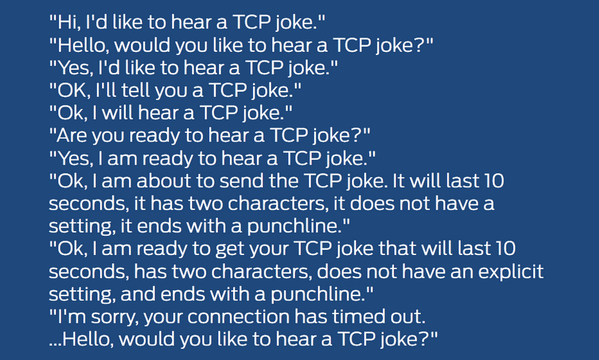
\includegraphics[width = \textwidth]{TCP.png}
\\
\\
7. Was kann man mit Hilfe von DNS ermitteln?
\\
\\
Das Domain-Name-System wird genutzt um die  ipv4 oder ipv6 namen f\"ur Lesbare Adressen(www) abzufragen. 
\\
\\
8. Wozu benötigt man URIs (bzw. URLs)?
\\
\\
Uniform-Recource-Locator gibt eine eindeutige Bezeichnung f\"ur Webobjekte.\\
Lokatoren: ".de/ordner/unterordner"(muss nicht so umgesetzt werden, kann auf andersartige Strukturen abgebildet werden.). (/#tag gibt eine Stelle auf der Page an, "raeume/ebene5?x=305,y=208" \"ubergibt Parameter).

\\
\\
9. Welchen grundsätzlichen Aufbau hat HTTP?
\\
\\
ASCII-basiertes Client-/Server-Modell\\
hat
n-buchstabige Kommandos (+ Parameter):\\
GET\\
PUT\\
POST\\
DELETE ...\\
\\
• 3-ziffrige Antwortcodes (+ Kommentare)\\
1xx noch in Arbeit\\
2xx o.k.\\
3xx sinnvolle Anfrage, aber keine Antwort\\
4xx Client-Fehler\\
5xx Server-Fehler\\
\\
\\
10. Was sind Web-Proxies?
\\
\\
Eine Art Internetpuffer.\\
Var1:Domains k\"onnen so Pages offserver anbieten um lokale anfragen lokal zu verwalten.\\
Var2: Browser k\"onnen einen Proxy vorschalten, der Anfragen an Server versendet, und erhaltene Dateien Weiterleitet.\\
Var3: Man-in-the-Middle-Scenario(bei Mobilfunk \"ublich). Transparenter Proxy der dem client vormacht direkt verbunden zu sein.
Var 4: Reverse Proxy. Content Provider besitzt „Reverse Proxy“ der Anfragen ggf. zum load balancing an verschiedene Server schickt. 

\end{document}